\documentclass[../report.tex]{subfiles}
\begin{document}
\graphicspath{{img/}{../img/}}

The architecture of the Data Access Layer, DAL, (See figure \ref{fig:DALclassdiagram}) has been implemented to satisfy NFR-07 and NFR-08, which state that it must be possible to add support for new types of media and to add new functionality. The DAL is build with a bridge pattern. This was done so that persistence modules can be swapped without changes in the layer above. If the persistence needs to be updated or changed to another technology, the new implementation can simply be dependency injected. Another important feature is that the DAL is generic. This facilitates being able to add a new entity in the database, without having to change the DALs bridge or interfaces.

A relational database management module has been implemented using Entity Framework (EF). EF is a good choice as it supports easy access to the database. The performance of EF is not as good as hard coded SQL-queries, but it is much more flexible and dynamic. The EFStorageConnection implementation uses the transaction state pattern to ensure that the database is consistent. The state pattern keeps track of the states of the entities, and only when Save Changes is invoked, the data is actually saved to the database.

\begin{figure}[H]
\centering
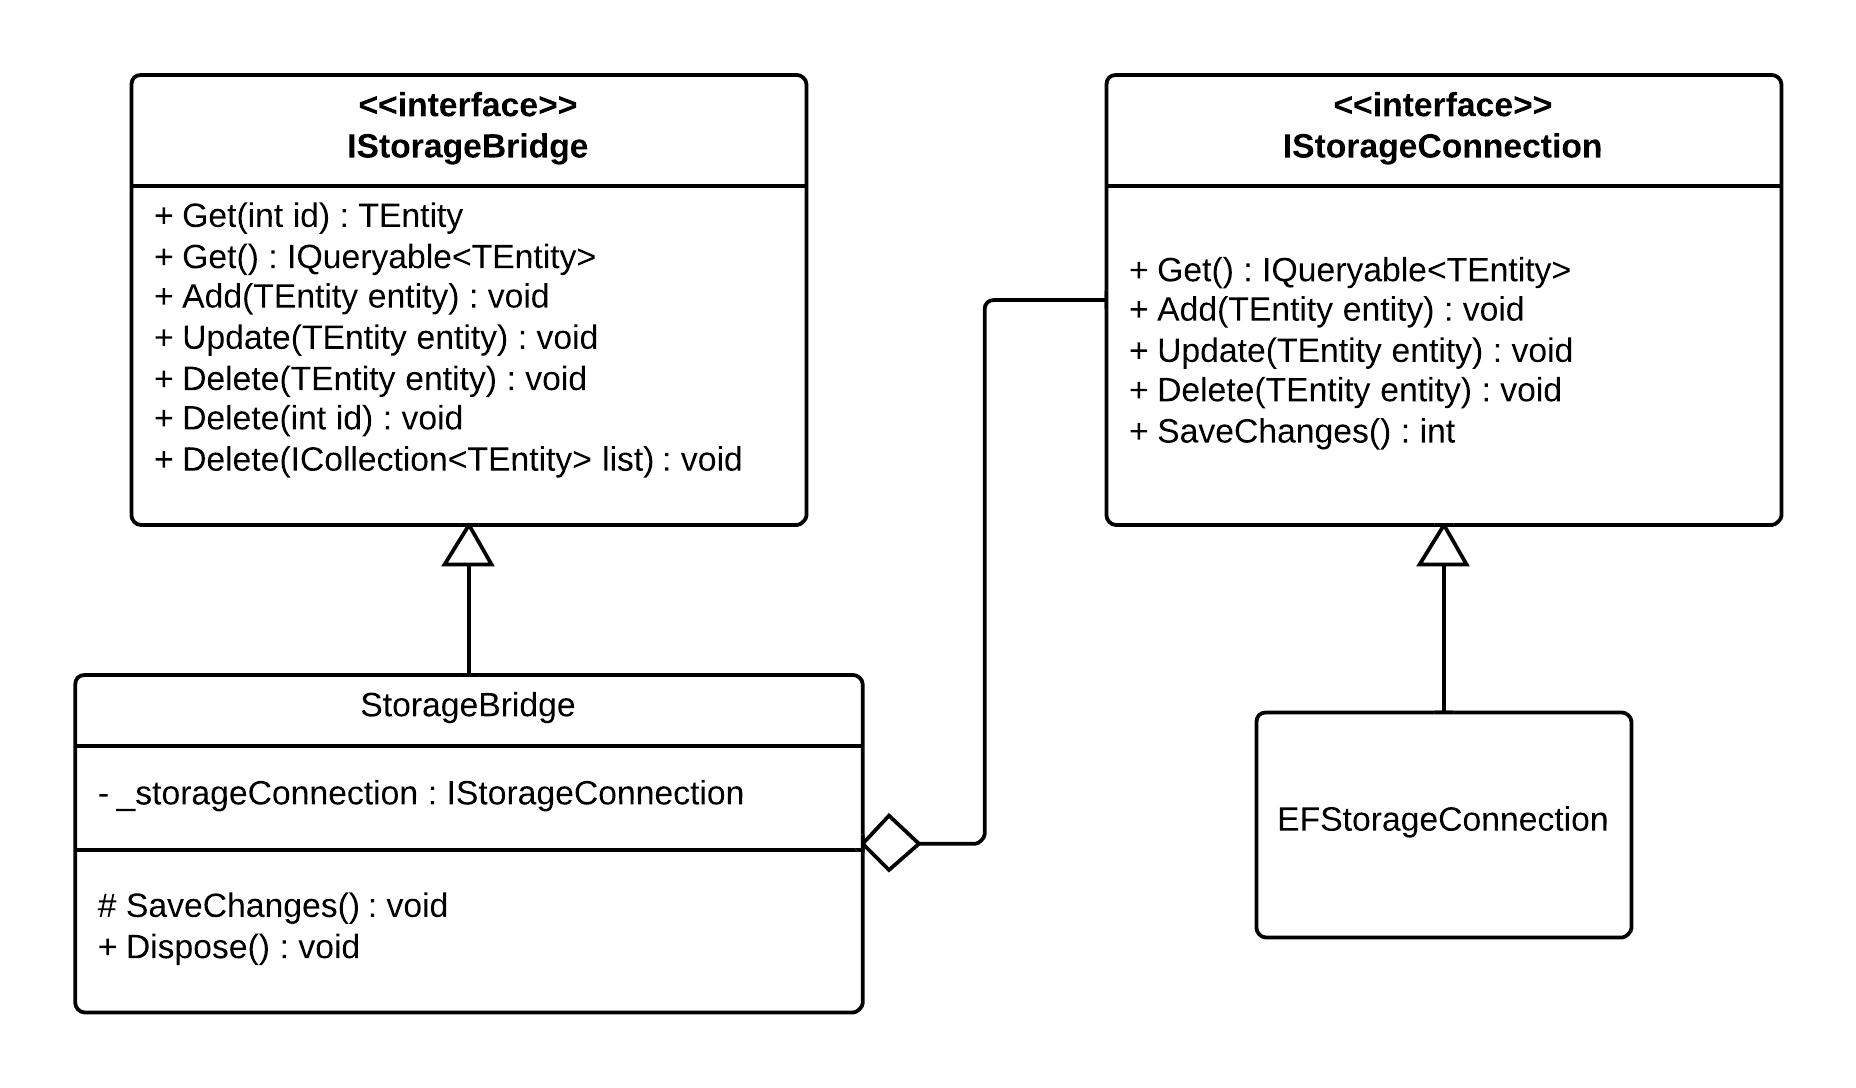
\includegraphics[width=\linewidth]{DALclassdiagram.png}
\caption{Data Access Layer architecture}
\label{fig:DALclassdiagram}
\end{figure} 

\end{document}